\documentclass{beamer}
\usepackage[utf8]{inputenc}

\usetheme{Madrid}
\usecolortheme{default}
\usepackage{amsmath,amssymb,amsfonts,amsthm}
\usepackage{txfonts}
\usepackage{tkz-euclide}
\usepackage{listings}
\usepackage{adjustbox}
\usepackage{array}
\usepackage{tabularx}
\usepackage{gvv}
\usepackage{lmodern}
\usepackage{circuitikz}
\usepackage{tikz}
\usepackage{graphicx}

\setbeamertemplate{page number in head/foot}[totalframenumber]

\usepackage{tcolorbox}
\tcbuselibrary{minted,breakable,xparse,skins}



\definecolor{bg}{gray}{0.95}
\DeclareTCBListing{mintedbox}{O{}m!O{}}{%
  breakable=true,
  listing engine=minted,
  listing only,
  minted language=#2,
  minted style=default,
  minted options={%
    linenos,
    gobble=0,
    breaklines=true,
    breakafter=,,
    fontsize=\small,
    numbersep=8pt,
    #1},
  boxsep=0pt,
  left skip=0pt,
  right skip=0pt,
  left=25pt,
  right=0pt,
  top=3pt,
  bottom=3pt,
  arc=5pt,
  leftrule=0pt,
  rightrule=0pt,
  bottomrule=2pt,
  toprule=2pt,
  colback=bg,
  colframe=orange!70,
  enhanced,
  overlay={%
    \begin{tcbclipinterior}
    \fill[orange!20!white] (frame.south west) rectangle ([xshift=20pt]frame.north west);
    \end{tcbclipinterior}},
  #3,
}
\lstset{
    language=C,
    basicstyle=\ttfamily\small,
    keywordstyle=\color{blue},
    stringstyle=\color{orange},
    commentstyle=\color{green!60!black},
    numbers=left,
    numberstyle=\tiny\color{gray},
    breaklines=true,
    showstringspaces=false,
}
%------------------------------------------------------------
%This block of code defines the information to appear in the
%Title page
\title %optional
{2.8.12}
\date{October 3,2025}


\author 
{Josyula G S Avaneesh - EE25BTECH11030}



\begin{document}



\frame{\titlepage}
\begin{frame}{Question}
Show that the tangent of an angle between the lines
$$\frac{x}{a}+\frac{y}{b}=1$$
$$\frac{x}{a}-\frac{y}{b}=1$$
is $\dfrac{2ab}{a^2-b^2}$
\end{frame}



\begin{frame}{Equation}
\textbf{Property:} The cosine of the angle between line 1 and line 2 is given by $\dfrac{{n_1}^\top n_2}{\norm{n_1}\norm{n_2}} $.
\end{frame}
\begin{frame}{Theoretical Solution}

Given details:
\begin{align}
   \myvec{\dfrac{1}{a}&&\dfrac{1}{b}}\vec{x}=1\\
   \myvec{\dfrac{1}{a}&&\dfrac{-1}{b}}\vec{x}=1
\end{align}
\end{frame}

\begin{frame}{Theoretical Solution}

Let the angle between the lines be $\theta$.
\begin{align}
  \cos\theta=\dfrac{{\myvec{\frac{1}{a}&&\frac{1}{b}}}^\top \myvec{\frac{1}{a} && \frac{-1}{b}}}{{\norm{\myvec{\frac{1}{a}&&\frac{1}{b}}}}\norm{\myvec{\frac{1}{a}&&\frac{-1}{b}}}}\\
   \cos\theta=\frac{\frac{1}{a^2}-\frac{1}{b^2}}{\sqrt{\brak{{\frac{1}{a}}^2}+\brak{\frac{1}{b}}^2}\sqrt{\brak{{\frac{1}{a}}^2}+\brak{\frac{-1}{b}}^2}}\\
   \cos\theta=\frac{b^2-a^2}{a^2+b^2}
\end{align}
\end{frame}


\begin{frame}{Theoretical Solution} 
\begin{align}
   \cos\theta=\frac{b^2-a^2}{a^2+b^2}
   \brak{\because \tan\theta=\frac{\sqrt{1-\cos^2\theta}}{\cos\theta}}\\
   \tan\theta=\left|\frac{2ab}{b^2-a^2}\right|
\end{align}
$\therefore$ The tan of the acute angle between the lines is $\dfrac{2ab}{a^2-b^2}$.

\end{frame}


\begin{frame}[fragile]
    \frametitle{C Code (1) - Function to store the points }

    \begin{lstlisting}

#include <math.h>

double calculate_tangent(double a, double b) {
    // Calculate the denominator of the formula.
    double denominator = (a * a) - (b * b);

    // Check if the denominator is zero. This happens when the lines are
    // perpendicular, and the tangent would be undefined (division by zero).
    if (denominator == 0.0) {
        return NAN; // Return "Not a Number" to indicate an undefined result.
    }


    \end{lstlisting}
\end{frame}

\begin{frame}[fragile]
    \frametitle{C Code (1) - Function to store the points }

    \begin{lstlisting}

    // Calculate the numerator.
    double numerator = 2.0 * a * b;

    // Return the final calculated tangent.
    return numerator / denominator;
}

    \end{lstlisting}
\end{frame}


\begin{frame}[fragile]
    \frametitle{Python Code - Using Shared Object}
    \begin{lstlisting}

import ctypes
import math
import numpy as np
import matplotlib.pyplot as plt

# Load the shared object
tangent_lib = ctypes.CDLL("./func.so")

# Define the C function's argument and return types
tangent_lib.calculate_tangent.argtypes = [ctypes.c_double, ctypes.c_double]
tangent_lib.calculate_tangent.restype = ctypes.c_double

# Create a Python-callable function
calculate_tangent = tangent_lib.calculate_tangent


\end{lstlisting}
\end{frame}

\begin{frame}[fragile]
    \frametitle{Python Code - Using Shared Object}
    \begin{lstlisting}
def plot_lines(a, b, tangent_value):
    """
    Plots the two lines and displays the tangent of the angle between them.
    """
    # Create a range of x-values for the plot.
    x_range = np.linspace(-abs(a) * 1.5, abs(a) * 1.5, 400)

    # Calculate the corresponding y-values for each line's equation.
    # Line 1: y = b * (1 - x/a)
    y1 = b * (1 - x_range / a)
    # Line 2: y = b * (x/a - 1)
    y2 = b * (x_range / a - 1)


\end{lstlisting}
\end{frame}
\begin{frame}[fragile]
    \frametitle{Python Code - Using Shared Object}
    \begin{lstlisting}


# Create the plot figure.
    plt.figure(figsize=(8, 8))
    plt.plot(x_range, y1, label=f'x/{a} + y/{b} = 1', color='blue')
    plt.plot(x_range, y2, label=f'x/{a} - y/{b} = 1', color='red')

    
# Add plot enhancements for better visualization.
    plt.axhline(0, color='black', linewidth=0.7)
    plt.axvline(0, color='black', linewidth=0.7)
    plt.grid(True, which='both', linestyle='--', linewidth=0.5)
    plt.legend()






\end{lstlisting}
\end{frame}

\begin{frame}[fragile]
     \frametitle{Python Code - Using Shared Object}
     \begin{lstlisting}
    plt.xlabel("x-axis")
    plt.ylabel("y-axis")
    plt.axis('equal')  # Use 'equal' scaling to ensure angles are not distorted.
# Set the plot title based on the tangent calculation result.
    if math.isnan(tangent_value):
        title = "Plot of the Lines\nTangent is undefined (lines are perpendicular)"
    else:
        title = f"Plot of the Lines\nTangent of the angle = {tangent_value:.4f}"
    plt.title(title)
    plt.savefig('figs/line.png')

    # Display the plot.
    plt.show()

     \end{lstlisting}
     \end{frame}

\begin{frame}[fragile]
     \frametitle{Python Code - Using Shared Object}
     \begin{lstlisting}
    def main():
    """
    Main function to define parameters, call the C function, and trigger the plot.
    """
    # Hardcoded values for 'a' and 'b'.
    a = 4.0
    b = 2.0

    # Call the C function with the hardcoded values.
    result = calculate_tangent(a, b)

    # Plot the lines using the results.
    plot_lines(a, b, result)


if __name__ == "__main__":
    main()

     \end{lstlisting}
     \end{frame}



\begin{frame}{Plot-Using Both C and Python}
    \centering
    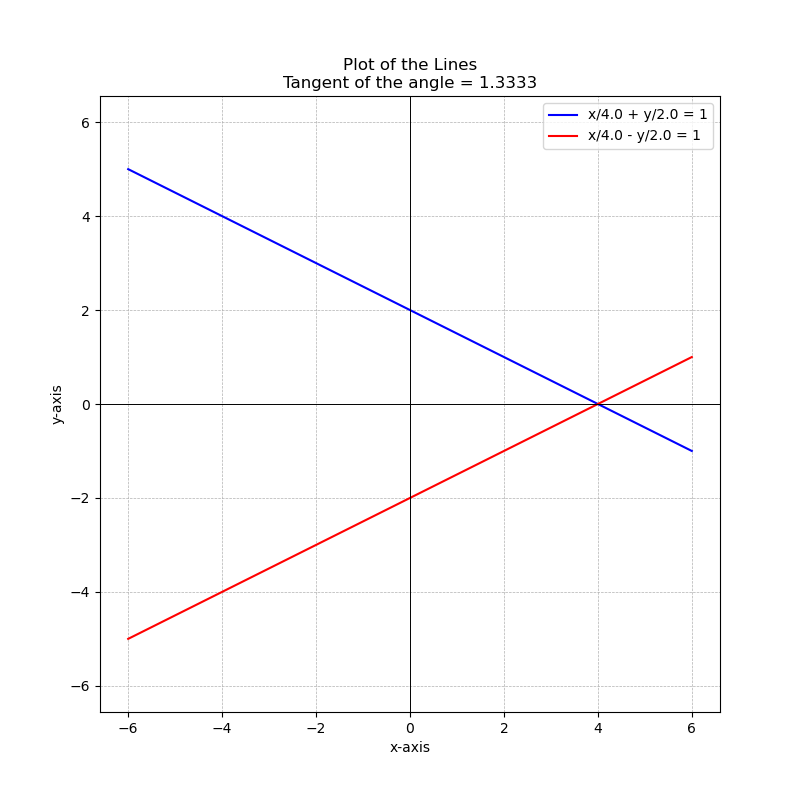
\includegraphics[width=\columnwidth, height=0.8\textheight, keepaspectratio]{figs/line.png}     
\end{frame}

\begin{frame}[fragile]
    \frametitle{Python Code}
    \begin{lstlisting}
import math
import numpy as np
import matplotlib.pyplot as plt


def calculate_tangent_py(a, b):
    """
    Calculates the tangent of the angle between the two lines directly in Python.
    The formula is derived from the slopes of the lines x/a + y/b = 1 and x/a - y/b = 1.
    """
    # Calculate the denominator of the tangent formula.
    denominator = a**2 - b**2

   


\end{lstlisting}
\end{frame}

\begin{frame}[fragile]
    \frametitle{Python Code }
    \begin{lstlisting}
 # Check for division by zero, which occurs when a = b or a = -b.
    # In this case, the lines are perpendicular, and the tangent is undefined.
    if denominator == 0:
        return math.nan  # Return Not-a-Number for an undefined tangent.

    # Calculate the numerator.
    numerator = 2 * a * b

    return numerator / denominator


\end{lstlisting}
\end{frame}

\begin{frame}[fragile]
    \frametitle{Python Code }
    \begin{lstlisting}
def plot_lines(a, b, tangent_value):
    """
    Plots the two lines and displays the tangent of the angle between them.
    """
    # Create a range of x-values for the plot.
    x_range = np.linspace(-abs(a) * 1.5, abs(a) * 1.5, 400)

    # Calculate the corresponding y-values for each line's equation.
    # Line 1: y = b * (1 - x/a)
    y1 = b * (1 - x_range / a)
    # Line 2: y = b * (x/a - 1)
    y2 = b * (x_range / a - 1)

    

\end{lstlisting}
\end{frame}

\begin{frame}[fragile]
    \frametitle{Python Code }
    \begin{lstlisting}
# Create the plot figure.
    plt.figure(figsize=(8, 8))
    plt.plot(x_range, y1, label=f'x/{a} + y/{b} = 1', color='blue')
    plt.plot(x_range, y2, label=f'x/{a} - y/{b} = 1', color='red')

# Add plot enhancements for better visualization.
    plt.axhline(0, color='black', linewidth=0.7)
    plt.axvline(0, color='black', linewidth=0.7)
    plt.grid(True, which='both', linestyle='--', linewidth=0.5)
    plt.legend()
    plt.xlabel("x-axis")
    plt.ylabel("y-axis")
    plt.axis('equal')  # Use 'equal' scaling to ensure angles are not distorted.

    

\end{lstlisting}
\end{frame}

\begin{frame}[fragile]
    \frametitle{Python Code }
    \begin{lstlisting}
# Set the plot title based on the tangent calculation result.
    if math.isnan(tangent_value):
        title = "Plot of the Lines\nTangent is undefined (lines are perpendicular)"
    else:
        title = f"Plot of the Lines\nTangent of the angle = {tangent_value:.4f}"
    plt.title(title)
    plt.savefig('figs/line2.png')

    # Display the plot.
    plt.show()

    

\end{lstlisting}
\end{frame}

\begin{frame}[fragile]
    \frametitle{Python Code }
    \begin{lstlisting}
def main():
    """
    Main function to define parameters, call the Python function, and trigger the plot.
    """
    # Hardcoded values for 'a' and 'b'.
    a = 4.0
    b = 2.0

    # Call the Python function with the hardcoded values.
    result = calculate_tangent_py(a, b)

    # Plot the lines using the results.
    plot_lines(a, b, result)


if __name__ == "__main__":
    main()

\end{lstlisting}
\end{frame}




\begin{frame}{Plot-Using only Python}
    \centering
    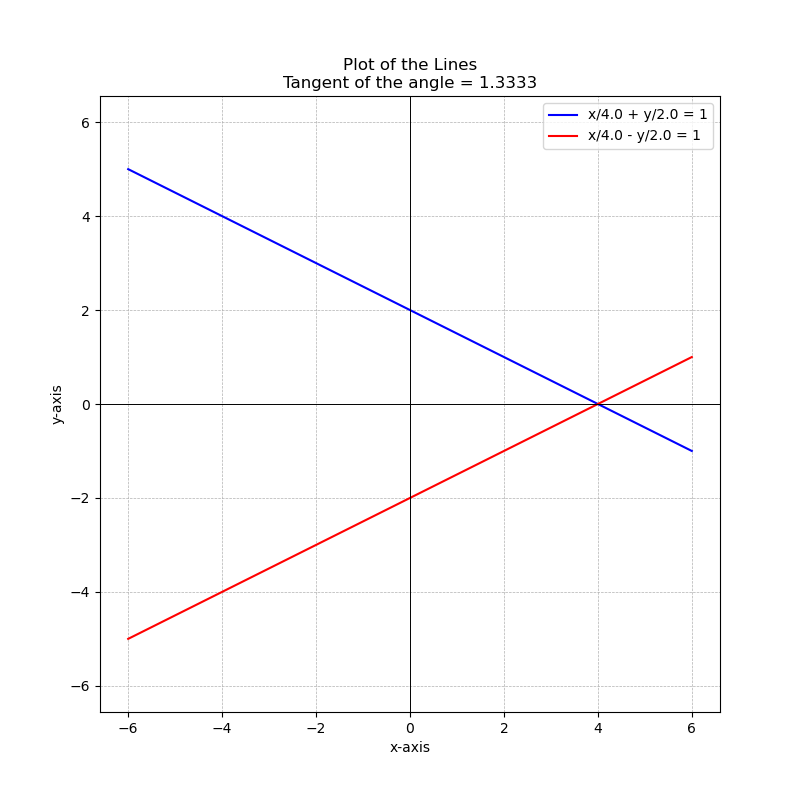
\includegraphics[width=\columnwidth, height=0.8\textheight, keepaspectratio]{figs/line2.png}     
\end{frame}


\end{document}